%%%%%%%%%%%%%%%%%%%%%%%%%%%%%%%%%%%%%%%%%
% Arsclassica Article
% LaTeX Template
% Version 1.1 (10/6/14)
%
% This template has been downloaded from:
% http://www.LaTeXTemplates.com
%
% Original author:
% Lorenzo Pantieri (http://www.lorenzopantieri.net) with extensive modifications by:
% Vel (vel@latextemplates.com)
%
% License:
% CC BY-NC-SA 3.0 (http://creativecommons.org/licenses/by-nc-sa/3.0/)
%
%%%%%%%%%%%%%%%%%%%%%%%%%%%%%%%%%%%%%%%%%

%----------------------------------------------------------------------------------------
%	PACKAGES AND OTHER DOCUMENT CONFIGURATIONS
%----------------------------------------------------------------------------------------

\documentclass[
10pt, % Main document font size
letterpaper, % Paper type, use 'letterpaper' for US Letter paper
oneside, % One page layout (no page indentation)
%twoside, % Two page layout (page indentation for binding and different headers)
headinclude,footinclude, % Extra spacing for the header and footer
english
]{article}

%%%%%%%%%%%%%%%%%%%%%%%%%%%%%%%%%%%%%%%%%
% Arsclassica Article
% Structure Specification File
%
% This file has been downloaded from:
% http://www.LaTeXTemplates.com
%
% Original author:
% Lorenzo Pantieri (http://www.lorenzopantieri.net) with extensive modifications by:
% Vel (vel@latextemplates.com)
%
% License:
% CC BY-NC-SA 3.0 (http://creativecommons.org/licenses/by-nc-sa/3.0/)
%
%%%%%%%%%%%%%%%%%%%%%%%%%%%%%%%%%%%%%%%%%

%----------------------------------------------------------------------------------------
%	REQUIRED PACKAGES
%----------------------------------------------------------------------------------------

\usepackage[
nochapters, % Turn off chapters since this is an article        
beramono, % Use the Bera Mono font for monospaced text (\texttt)
eulermath,% Use the Euler font for mathematics
pdfspacing, % Makes use of pdftex’ letter spacing capabilities via the microtype package
dottedtoc % Dotted lines leading to the page numbers in the table of contents
]{classicthesis} % The layout is based on the Classic Thesis style

\usepackage{arsclassica} % Modifies the Classic Thesis package

\usepackage[T1]{fontenc} % Use 8-bit encoding that has 256 glyphs

\usepackage[utf8]{inputenc} % Required for including letters with accents

\usepackage{graphicx} % Required for including images
\graphicspath{{Figures/}} % Set the default folder for images

\usepackage{enumitem} % Required for manipulating the whitespace between and within lists

\usepackage{lipsum} % Used for inserting dummy 'Lorem ipsum' text into the template

\usepackage{subfig} % Required for creating figures with multiple parts (subfigures)

\usepackage{amsmath,amssymb,amsthm} % For including math equations, theorems, symbols, etc

\usepackage{varioref} % More descriptive referencing

%----------------------------------------------------------------------------------------
%	THEOREM STYLES
%---------------------------------------------------------------------------------------

\theoremstyle{definition} % Define theorem styles here based on the definition style (used for definitions and examples)
\newtheorem{definition}{Definition}

\theoremstyle{plain} % Define theorem styles here based on the plain style (used for theorems, lemmas, propositions)
\newtheorem{theorem}{Theorem}

\theoremstyle{remark} % Define theorem styles here based on the remark style (used for remarks and notes)

%----------------------------------------------------------------------------------------
%	HYPERLINKS
%---------------------------------------------------------------------------------------

\hypersetup{
%draft, % Uncomment to remove all links (useful for printing in black and white)
colorlinks=true, breaklinks=true, bookmarks=true,bookmarksnumbered,
urlcolor=webbrown, linkcolor=RoyalBlue, citecolor=webgreen, % Link colors
pdftitle={}, % PDF title
pdfauthor={\textcopyright}, % PDF Author
pdfsubject={}, % PDF Subject
pdfkeywords={}, % PDF Keywords
pdfcreator={pdfLaTeX}, % PDF Creator
pdfproducer={LaTeX with hyperref and ClassicThesis} % PDF producer
} % Include the structure.tex file which specified the document structure and layout
\usepackage[letterpaper]{geometry}
\geometry{verbose,tmargin=1in,bmargin=1.5in,lmargin=1.5in,rmargin=1.5in}

\hyphenation{Fortran hy-phen-ation} % Specify custom hyphenation points in words with dashes where you would like hyphenation to occur, or alternatively, don't put any dashes in a word to stop hyphenation altogether

%----------------------------------------------------------------------------------------
%	TITLE AND AUTHOR(S)
%----------------------------------------------------------------------------------------

\title{\normalfont\spacedallcaps{CIS 559 Project 1:\break Parallel Football}} % The article title

\author{\spacedlowsmallcaps{Ian Sibner, Derick Olson, Spriha Baruah, Anthony Hsieh}} % The article author(s) - author affiliations need to be specified in the AUTHOR AFFILIATIONS block

\date{19 September 2015} % An optional date to appear under the author(s)

%----------------------------------------------------------------------------------------

\begin{document}

%----------------------------------------------------------------------------------------
%	HEADERS
%----------------------------------------------------------------------------------------

\renewcommand{\sectionmark}[1]{\markright{\spacedlowsmallcaps{#1}}} % The header for all pages (oneside) or for even pages (twoside)
%\renewcommand{\subsectionmark}[1]{\markright{\thesubsection~#1}} % Uncomment when using the twoside option - this modifies the header on odd pages
\lehead{\mbox{\llap{\small\thepage\kern1em\color{halfgray} \vline}\color{halfgray}\hspace{0.5em}\rightmark\hfil}} % The header style

\pagestyle{scrheadings} % Enable the headers specified in this block

%----------------------------------------------------------------------------------------
%	TABLE OF CONTENTS & LISTS OF FIGURES AND TABLES
%----------------------------------------------------------------------------------------

\maketitle % Print the title/author/date block

\setcounter{tocdepth}{2} % Set the depth of the table of contents to show sections and subsections only

\tableofcontents % Print the table of contents

\listoffigures % Print the list of figures

% \listoftables % Print the list of tables

%----------------------------------------------------------------------------------------
%	ABSTRACT
%----------------------------------------------------------------------------------------

\section{Introduction} % This section will not appear in the table of contents due to the star (\section*)

\lipsum[1] % Dummy text

\section{Initial Insights and Observations}

\lipsum[3]

\section{Strategies and Concepts}
\subsection {Global scope}

Given the loose efficiency constraints given the problem, we decided that a globally optimal benefit function would be both feasible and desirable. The primary gain from this decision was a team optimized for late gameplay, where our players were able to seek out and steal balls toward the end of the game. The reason was that once we and other teams cleared the balls near our respective goals, balls became scarce. If any team had accumulated balls, even if they were far from our players, they would seek them out and attempt to score with them.

On the other hand, as teams improved, the game time grew shorter and quicker. In such a game, it is possible that a globally optimal zone will change into a depleted zone before a far-away team can reach it. It is likely that our model did not fully capture the constantly changing state of the game board. We addressed this by heavily weighting our own goal in benefit calculations.

\subsection{Cell clustering}
On the second iteration of our benefit function, we accounted for ball and opponent clustering by keeping track of the number of balls and opponents surrounding a particular cell. This allowed our players to seek out areas of high benefit, rather than single cells. 

After initial trials with a large radius, we settled on a radius of 3. We observed that larger radii caused the players to move back and forth somewhat inefficiently, and hypothesize that these larger zones changed too quickly for players to capitalize on them.


\section{Implementation}


Reference to Figure~\vref{fig:gallery}. % The \vref command specifies the location of the reference

\begin{figure}[tb]
\centering 
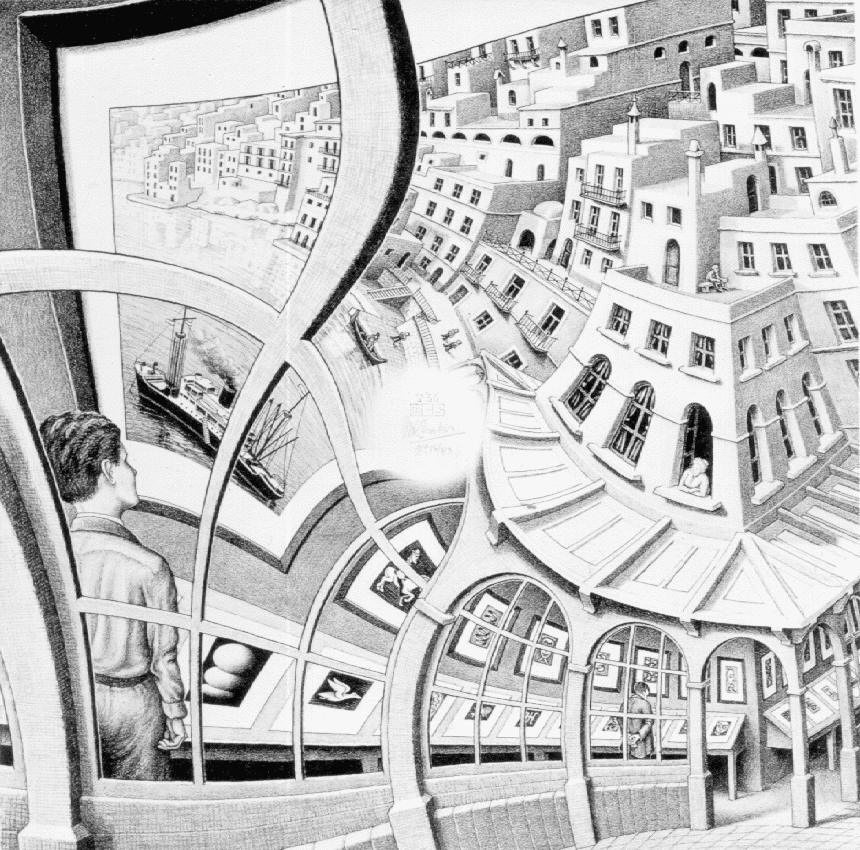
\includegraphics[width=0.5\columnwidth]{GalleriaStampe} 
\caption[An example of a floating figure]{An example of a floating figure (a reproduction from the \emph{Gallery of prints}, M.~Escher,\index{Escher, M.~C.} from \url{http://www.mcescher.com/}).} % The text in the square bracket is the caption for the list of figures while the text in the curly brackets is the figure caption
\label{fig:gallery} 
\end{figure}

\section{Results}

\lipsum[3]

\section{Contributions}

\lipsum[2]

\section{Future Directions and Limitations}

\subsection{Generalized Step Distance}
This idea stems from our attempts to take advantage of global-scope “hotspots,” or high-density ball clusters that are not near the goal. The existing implementation weights balls close to the home goal particularly high, which is good in the early game, but may not be ideal overall. 

As we can see in the figure above, certain strategies tend to cluster balls near an opponent goal, where they stay relatively untouched for several cycles. A smarter global-cluster detection would drop the current strategy 

The biggest disadvantage to this approach is that the time it takes to travel to such a cluster may be greater than the the time the cluster exists. Even if the seeking team is able to reach the cluster in time, the balls lost in the transit time may not be worth it.

It would be possible to determine, by factoring in the number of balls left $B_{total}$, the number of balls in close range $B_{nearby}$, and the number of balls expected to remain in the cluster $B_{cluster}$. Such a strategy would decide to go for the cluster if and only if: 
$$B_{total} - B_{nearby} < B_{cluster}$$

One way of implementing this strategy would be to generalize the  \texttt{numberOfStepsToGoal()} benefit function to be \texttt{numberOfStepsToPosition(p)}, where the latter takes in any valid position $p$ as it’s argument, causing the cells around it to get a score boost. Then, upon deciding to pursue a cluster, this position would be updated to the cluster center, until a new position was found.

\section{Acknowledgments}

Our progress was largely a result of the class discussions and adopted strategies. Through the course of the project, we adopted starting strategies from Groups 1 (Grid Player), as well as experiments in stealing opponent balls with the opening placements. We would like to give special thanks to Groups 2 and 6 for the important heuristics we adopted from them and eventually used in our final implementation. 

Group 2 (The Swarm) was the first group to successfully implement a kind of benefit function with the emergent behavior of a bucket brigade. This function was based on the number of steps from the ball to the goal, and we adopted it as a core feature of our ensemble benefit function.

Group 6 (Bucket Brigade) contributed a smarter kicking function that favored passing to players over kicking as far to the goal as possible. We adopted this function as a core part of our improved kicking strategy.

\section{Conclusion}

\lipsum[1]

\subsection{Figure Composed of Subfigures}

Reference the figure composed of multiple subfigures as Figure~\vref{fig:esempio}. Reference one of the subfigures as Figure~\vref{fig:ipsum}. % The \vref command specifies the location of the reference

\begin{figure}[tb]
\centering
\subfloat[A city market.]{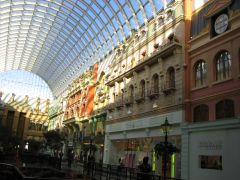
\includegraphics[width=.45\columnwidth]{Lorem}} \quad
\subfloat[Forest landscape.]{
\includegraphics[width=.45\columnwidth]{Ipsum}\label{fig:ipsum}} \\
\subfloat[Mountain landscape.]{
\includegraphics[width=.45\columnwidth]{Dolor}} \quad
\subfloat[A tile decoration.]{
\includegraphics[width=.45\columnwidth]{Sit}}
\caption[A number of pictures.]{A number of pictures with no common theme.} % The text in the square bracket is the caption for the list of figures while the text in the curly brackets is the figure caption
\label{fig:esempio}
\end{figure}

%----------------------------------------------------------------------------------------

\end{document}
